\documentclass[border=5pt]{standalone}
\usepackage[T1]{fontenc}
\usepackage{lmodern}
\usepackage{pgfplots}
\usepgfplotslibrary{groupplots}
\pgfplotsset{compat=1.18}
\begin{document}
\sffamily
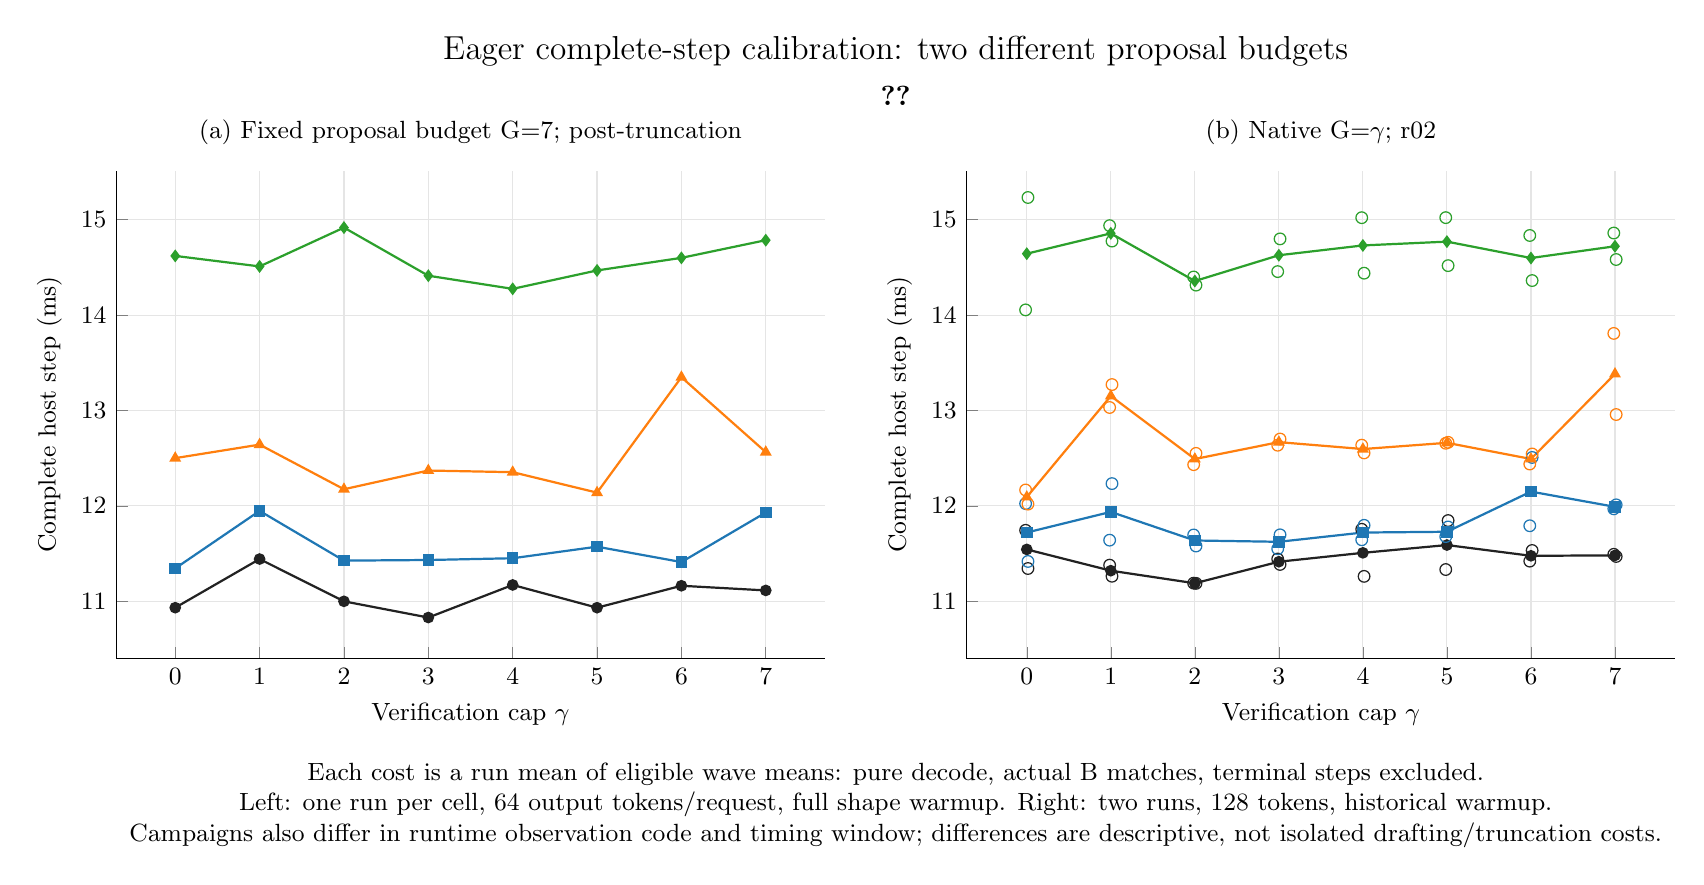
\begin{tikzpicture}
\definecolor{series0}{HTML}{222222}
\definecolor{series1}{HTML}{1f77b4}
\definecolor{series2}{HTML}{ff7f0e}
\definecolor{series3}{HTML}{2ca02c}
\definecolor{series4}{HTML}{d62728}
\definecolor{series5}{HTML}{9467bd}
\definecolor{series6}{HTML}{8c564b}
\definecolor{series7}{HTML}{e377c2}
\begin{groupplot}[group style={group size=2 by 1,horizontal sep=1.8cm},width=9.0cm,height=6.2cm,scale only axis,grid=major,grid style={gray!20},axis lines*=left,tick label style={font=\small},label style={font=\small},title style={font=\small},unbounded coords=jump,ymin=10.396533188266359,ymax=15.513617173333333]
\nextgroupplot[title={(a) Fixed proposal budget G=7; post-truncation},xlabel={Verification cap $\gamma$},ylabel={Complete host step (ms)},xtick={0,1,2,3,4,5,6,7},xticklabels={0,1,2,3,4,5,6,7},scaled y ticks=false,yticklabel style={/pgf/number format/fixed,/pgf/number format/precision=2},legend columns=4,legend to name=sharedlegend,legend style={draw=none,font=\small,/tikz/every even column/.append style={column sep=8pt}}]
\addplot+[color=series0,mark=*,mark size=1.7pt,mark options={fill=series0,draw=series0},line width=0.8pt] coordinates {(0,10.9330202802) (1,11.4429236735) (2,10.9996581271) (3,10.8297220711) (4,11.1712966416) (5,10.9329778991) (6,11.162753151) (7,11.1139294456)};
\addlegendentry{B=1}
\addplot+[only marks,forget plot,color=series0,mark=o,mark size=2.1pt,mark options={fill=white,line width=0.45pt}] coordinates {};
\addplot+[color=series1,mark=square*,mark size=1.7pt,mark options={fill=series1,draw=series1},line width=0.8pt] coordinates {(0,11.3449147399) (1,11.9478394942) (2,11.4262251893) (3,11.4328128807) (4,11.4512735851) (5,11.5724315623) (6,11.4111472679) (7,11.9305643061)};
\addlegendentry{B=4}
\addplot+[only marks,forget plot,color=series1,mark=o,mark size=2.1pt,mark options={fill=white,line width=0.45pt}] coordinates {};
\addplot+[color=series2,mark=triangle*,mark size=1.7pt,mark options={fill=series2,draw=series2},line width=0.8pt] coordinates {(0,12.5006231452) (1,12.64230003) (2,12.1745948053) (3,12.3705556585) (4,12.3534159823) (5,12.139028999) (6,13.3487191225) (7,12.563617047)};
\addlegendentry{B=16}
\addplot+[only marks,forget plot,color=series2,mark=o,mark size=2.1pt,mark options={fill=white,line width=0.45pt}] coordinates {};
\addplot+[color=series3,mark=diamond*,mark size=1.7pt,mark options={fill=series3,draw=series3},line width=0.8pt] coordinates {(0,14.6201394355) (1,14.5100856364) (2,14.9169395897) (3,14.4126840909) (4,14.2748159032) (5,14.4678544194) (6,14.5997474828) (7,14.7849923448)};
\addlegendentry{B=64}
\addplot+[only marks,forget plot,color=series3,mark=o,mark size=2.1pt,mark options={fill=white,line width=0.45pt}] coordinates {};
\nextgroupplot[title={(b) Native G=$\gamma$; r02},xlabel={Verification cap $\gamma$},ylabel={Complete host step (ms)},xtick={0,1,2,3,4,5,6,7},xticklabels={0,1,2,3,4,5,6,7},scaled y ticks=false,yticklabel style={/pgf/number format/fixed,/pgf/number format/precision=2}]
\addplot+[color=series0,mark=*,mark size=1.7pt,mark options={fill=series0,draw=series0},line width=0.8pt] coordinates {(0,11.5438464175) (1,11.3207841657) (2,11.1889618688) (3,11.4148614503) (4,11.5079741033) (5,11.5895325736) (6,11.4768334035) (7,11.481184956)};
\addplot+[only marks,forget plot,color=series0,mark=o,mark size=2.1pt,mark options={fill=white,line width=0.45pt}] coordinates {(-0.014,11.7439607837) (0.014,11.3437320513) (0.986,11.3789141884) (1.014,11.2626541429) (1.986,11.1900662496) (2.014,11.1878574879) (2.986,11.4433093586) (3.014,11.386413542) (3.986,11.7545870836) (4.014,11.2613611229) (4.986,11.3328777907) (5.014,11.8461873565) (5.986,11.4210773529) (6.014,11.5325894542) (6.986,11.4924740868) (7.014,11.4698958252)};
\addplot+[color=series1,mark=square*,mark size=1.7pt,mark options={fill=series1,draw=series1},line width=0.8pt] coordinates {(0,11.720914877) (1,11.937166264) (2,11.637343297) (3,11.6235811067) (4,11.7206626029) (5,11.7287642497) (6,12.149784483) (7,11.990073721)};
\addplot+[only marks,forget plot,color=series1,mark=o,mark size=2.1pt,mark options={fill=white,line width=0.45pt}] coordinates {(-0.014,12.0240834311) (0.014,11.4177463229) (0.986,11.640639979) (1.014,12.2336925489) (1.986,11.6952477809) (2.014,11.5794388132) (2.986,11.5503670333) (3.014,11.6967951801) (3.986,11.6449767043) (4.014,11.7963485015) (4.986,11.678257013) (5.014,11.7792714863) (5.986,11.791750323) (6.014,12.507818643) (6.986,11.9690365363) (7.014,12.0111109058)};
\addplot+[color=series2,mark=triangle*,mark size=1.7pt,mark options={fill=series2,draw=series2},line width=0.8pt] coordinates {(0,12.0928267123) (1,13.1515225633) (2,12.491281344) (3,12.6682687223) (4,12.5958152587) (5,12.6611565211) (6,12.4916238743) (7,13.3827238588)};
\addplot+[only marks,forget plot,color=series2,mark=o,mark size=2.1pt,mark options={fill=white,line width=0.45pt}] coordinates {(-0.014,12.1670425913) (0.014,12.0186108333) (0.986,13.0314439457) (1.014,13.2716011809) (1.986,12.4320618824) (2.014,12.5505008055) (2.986,12.6358114655) (3.014,12.7007259791) (3.986,12.6363693253) (4.014,12.5552611922) (4.986,12.6561440429) (5.014,12.6661689994) (5.986,12.4388640773) (6.014,12.5443836714) (6.986,13.8078763985) (7.014,12.9575713191)};
\addplot+[color=series3,mark=diamond*,mark size=1.7pt,mark options={fill=series3,draw=series3},line width=0.8pt] coordinates {(0,14.6434212976) (1,14.8564538636) (2,14.356632461) (3,14.6271805479) (4,14.7300058116) (5,14.7698274697) (6,14.5980765385) (7,14.7211726797)};
\addplot+[only marks,forget plot,color=series3,mark=o,mark size=2.1pt,mark options={fill=white,line width=0.45pt}] coordinates {(-0.014,14.0543904365) (0.014,15.2324521587) (0.986,14.9374475909) (1.014,14.7754601364) (1.986,14.3994203506) (2.014,14.3138445714) (2.986,14.4557272055) (3.014,14.7986338904) (3.986,15.0208557101) (4.014,14.439155913) (4.986,15.0213302424) (5.014,14.518324697) (5.986,14.8343922462) (6.014,14.3617608308) (6.986,14.8599257031) (7.014,14.5824196562)};
\end{groupplot}
\path (group c1r1.north west) -- node[above=1.2cm,font=\large] {Eager complete-step calibration: two different proposal budgets} (group c2r1.north east);
\path (group c1r1.north west) -- node[above=0.7cm] {\ref{sharedlegend}} (group c2r1.north east);
\path (group c1r1.south west) -- node[below=1.2cm,align=center,font=\small] {Each cost is a run mean of eligible wave means: pure decode, actual B matches, terminal steps excluded.\\Left: one run per cell, 64 output tokens/request, full shape warmup. Right: two runs, 128 tokens, historical warmup.\\Campaigns also differ in runtime observation code and timing window; differences are descriptive, not isolated drafting/truncation costs.} (group c2r1.south east);
\end{tikzpicture}
\end{document}
